\documentclass[fleqn,a4j,10pt]{jsarticle}
\usepackage{layout,url,resume}
\usepackage[dvipdfmx]{graphicx}
\usepackage{mathpartir}
\usepackage{amsmath,amssymb}
\usepackage{amsthm}
\usepackage{bussproofs}
\usepackage{syntax}
\pagestyle{empty}
\usepackage{multicol}


\begin{document}
%\layout

\title{Coqによる証明済み型検査器を用いた算術式インタプリタの実装}

% 和文著者名
\author{ Arch B2 nem }

\newcommand{\bnfdef}{::=}
\newcommand{\bs}{\boldsymbol}
\newlength{\len}
\settowidth{\len}{$\bnfdef$}
\newcommand{\bnfor}{\makebox[\len]{$|$}}

%\DeclareMathSymbol{\mhyph}{\mathalpha}{operators}{`-}

% 和文概要
\begin{abstract}
  「型システム入門」\cite{TaPL} 8章型付き算術式に定理証明支援家Coqを用いて証明し,OCamlを用いてパーサーをつけることで簡易的なインタプリタを実装した.
\end{abstract}

\maketitle
\thispagestyle{empty}

\section{経緯}
以前から興味を持っていた型理論や圏論が定理証明支援系によって形式的な証明がなされていることを知り,定理証明支援系であるCoqをやってみた.\par
CoqはSoftware Foundations\cite{SF}(以下SF)の有志による日本語翻訳版\cite{sfja}を用いて学んだ. SFは4巻ありそれぞれ,1巻はCoq,2巻はプログラミング言語論の形式化,3巻はアルゴリズムの形式化,4巻は形式手法の解説という構成になっており,2巻まで終わらせた. その後,型理論の解説書である「型システム入門」をCoqを用いて形式化を始めた.その際,SF2巻にはなかった型推論の形式化とそのインタプリタの実装を最終目標として設定し,今学期は型付きラムダ計算の型検査器の形式化とそのインタプリタの実装を目標として設定した.\par

\section{ツール}
\subsection{定理証明支援系Coq}
定理証明支援系とは,型理論と証明論の対応であるカリー=ハワード同型対応を基にしてコンピュータ上での形式的な証明を可能とするためのシステムである. 定理証明支援系には,Agda,Lean,Idris,Isabelle,F*などといったものもある. その中でCoqは上記のSFを含め日本語による資料が他の支援系に比べて多いことから今回はCoqを選んだ. \par
\subsection{OCaml}
Coqで記述・証明した関数を他の言語に変換するExtranctionという拡張機能を用いて,式の評価を行う関数及び型付けを行う関数をOCamlに変換,OCamlで記述したレキサー及びパーサーを用いてこれらの関数の実行環境を実装した.\par
なお,OCamlでの実装には字句解析器生成器ocamllex, 構文解析器生成器Menhir, ビルドシステムDuneを使用した.\\
\begin{figure}[htbp]
    \begin{center}
        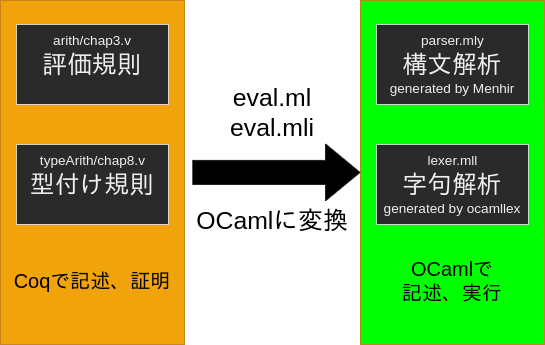
\includegraphics[width=6cm]{wip.png}
        \caption{構成}
        \label{sample}
    \end{center}
\end{figure}


\section{構文}
型付き算術式の構文を以下に記す.\\

\begin{eqnarray*}
  \mbox{Term} &\bnfdef& \\
  &\bnfor& \mbox{true}\ \\
  &\bnfor& \mbox{false}\ \\
  &\bnfor& \mbox{0}\ \\
  &\bnfor& \mbox{succ Term}\ \\
  &\bnfor& \mbox{pred Term}\ \\
  &\bnfor& \mbox{iszero Term}\ \\
  &\bnfor& \mbox{if Term then Term else Term}\ \\
\end{eqnarray*}

\begin{eqnarray*}
  \mbox{Value} &\bnfdef& \\
  &\bnfor& \mbox{true}\ \\
  &\bnfor& \mbox{false}\ \\
  &\bnfor& \mbox{NatValue}\ \\
\end{eqnarray*}

\begin{eqnarray*}
  \mbox{NatValue} &\bnfdef& \\
  &\bnfor& \mbox{0}\ \\
  &\bnfor& \mbox{succ NatValue}\ \\
\end{eqnarray*}

\begin{eqnarray*}
  \mbox{Type} &\bnfdef& \\
  &\bnfor& \mbox{Bool}\ \\
  &\bnfor& \mbox{Nat}\ \\
\end{eqnarray*}

\section {評価規則}
tを評価するとt'となること(1ステップ評価) を $t \longrightarrow t'$と書く.また,評価の反射的推移的閉包(多ステップ評価)を $\longrightarrow*$ で表す.\\

\begin{prooftree}
    \AxiomC {$t1 \longrightarrow t1'$}
    \RightLabel {(E_If)}
    \UnaryInfC {$if$ $t1$ $t2$ $t3 \longrightarrow if$ $t1'$ $t2$ $t3$}
\end{prooftree}

\begin{prooftree}
    \AxiomC {}
    \RightLabel {(E_IfTrue)}
    \UnaryInfC {$if$ $true$ $t2$ $t3 \longrightarrow t2$}
\end{prooftree}

\begin{prooftree}
    \AxiomC {}
    \RightLabel {(E_IfFalse)}
    \UnaryInfC {$if$ $false$ $t2$ $t3 \to t3$}
\end{prooftree}

\begin{prooftree}
    \AxiomC {$t1 \longrightarrow t1'$}
    \RightLabel {(E_Succ)}
    \UnaryInfC {$succ$ $t1 \longrightarrow succ$ $t1'$}
\end{prooftree}

\begin{prooftree}
    \AxiomC {}
    \RightLabel {(E_PredZero)}
    \UnaryInfC {$pred$ $0 \longrightarrow 0$}
\end{prooftree}

\begin{prooftree}
    \AxiomC {NatValue nv1}
    \RightLabel {(E_PredSucc)}
    \UnaryInfC {$pred$ $succ$ $nv1 \longrightarrow nv1$}
\end{prooftree}

\begin{prooftree}
    \AxiomC {$t1 \longrightarrow t1'$}
    \RightLabel {(E_Pred)}
    \UnaryInfC {$pred$ $t1 \longrightarrow pred$ $t1'$}
\end{prooftree}

\begin{prooftree}
    \AxiomC {}
    \RightLabel {(E_IsZeroZero)}
    \UnaryInfC {$iszero$ $0 \longrightarrow true$}
\end{prooftree}

\begin{prooftree}
    \AxiomC {NatValue nv1}
    \RightLabel {(E_IsZeroSucc)}
    \UnaryInfC {$iszero$ $succ$ $nv1 \longrightarrow false$}
\end{prooftree}

\begin{prooftree}
    \AxiomC {$t1 \longrightarrow t1'$}
    \RightLabel {(E_IsZero)}
    \UnaryInfC {$iszero$ $t1 \longrightarrow iszero$ $t1'$}
\end{prooftree}

\subsection *{証明済みの性質}
評価規則の健全性を評価の決定性と停止性によって証明した.

\theoremstyle{definition}
\newtheorem *{theorem}{定理}
\begin {theorem}
    評価の決定性\par
    すべての項に対して評価は一意に定まる\par
    \(\forall\) t \(\forall\) t1 \(\forall\) t2
    $( t \longrightarrow t1 ) \land ( t \longrightarrow t2 ) \to t1 = t2 $
\end{theorem}
\newtheorem*{theorem*}{定理}
\begin{theorem}
    停止性\par
    すべての項に対して評価を進めると,ある正規形に達する.\par
    \(\forall\) t \(\exists\) t'
    $( t \longrightarrow * t')  \land  (\lnot \exists t''$ $t' \longrightarrow t'')$ 
\end{theorem}

その他,大ステップ評価を定義し,意味論の一致なども証明した.\\

\section{型付け規則}
項tが型Tに型付けされることを $t \colon T$ と書く.\\

\begin{prooftree}
    \AxiomC {}
    \RightLabel {(T_True)}
    \UnaryInfC {$true \colon Bool$}
\end{prooftree}

\begin{prooftree}
    \AxiomC {}
    \RightLabel {(T_False)}
    \UnaryInfC {$false \colon Bool$}
\end{prooftree}

\begin{prooftree}
    \AxiomC {$t1 \colon Bool$  $t2 \colon T$ $t3 \colon T$}
    \RightLabel {(T_If)}
    \UnaryInfC {$if$ $t1$ $t2$ $t3 \colon T$}
\end{prooftree}

\begin{prooftree}
    \AxiomC {}
    \RightLabel {(T_Zero)}
    \UnaryInfC {$0 \colon Nat$}
\end{prooftree}

\begin{prooftree}
    \AxiomC {$t1 \colon Nat$}
    \RightLabel {(T_Succ)}
    \UnaryInfC {$succ$ $t1 \colon Nat$}
\end{prooftree}

\begin{prooftree}
    \AxiomC {$t1 \colon Nat$}
    \RightLabel {(T_Pred)}
    \UnaryInfC {$pred$ $t1 \colon Nat$}
\end{prooftree}

\begin{prooftree}
    \AxiomC {$t1 \colon Nat$}
    \RightLabel {(T_IsZero)}
    \UnaryInfC {$iszero$ $t1 \colon Bool$}
\end{prooftree}

\bibliographystyle{junsrt}
\bibliography{resume}

\subsection *{証明済みの性質}
型付け規則の健全性は進行定理と保存定理によって証明を行った.\\
\begin {theorem}
    進行\par
    正しく型付けされた任意に項tは値であるか, $t \longrightarrow t'$ となるt'が存在する.\par
    \(\forall\) t \
     $(Value $ ${t)} \lor (\exists t', t \longrightarrow t' ) $
\end{theorem}

\begin{theorem}
    保存\par
    正しく型付けされた任意の項tと $t \longrightarrow t'$ となるt'は型が一致する.\par
    \(\forall\) t \(\forall\) t'
    $ (t \longrightarrow t')  \land (t \colon T) \to t' \colon T$
\end{theorem}

\section{まとめ}
今学期の目標であった型付きラムダ計算を証明,実装することはできなかった主な要因は本旨あまり関わらない性質についての証明に時間をかけたことやCoqにおいて証明しやすい定義が存在しその通りに記述することに不慣れであったこと,数学の知識が不足していたことなどが挙げられる.そのため,今後の形式化においては一定以上の時間をかけて証明できないあまり重要でない性質については飛ばすようにする.また,今学期の経験である程度Coqに慣れてきたので今後は進捗が生まれやすくなるだろう.

\section{今後}
「型システム入門」の形式化を進めて,来学期には型推論器の形式化を終えたい.\par
Coqの正しさを保証しているCICとZFCの互換性について理解をしたいので数学基礎論の知識をつける予定である.\par
Coqは可読性が低いので他の証明支援系を使うことも検討する.そのためにもAgdaを少し触れたい.\par

\begin{thebibliography}{}
\bibitem{TaPL} オーム社/Benjamin C. Pierce 著、住井 英二郎 監訳、遠藤 侑介 訳、酒井 政裕 訳、今井 敬吾 訳、黒木 裕介 訳、今井 宜洋 訳、才川隆文 訳、今井 健男 訳 https://www.ohmsha.co.jp/book/9784274069116/
\bibitem{SF} 「型システム入門」の作者Benjamin C. Pierce氏などによって継続的にメンテナンスされているCoqの教科書.\\
https://softwarefoundations.cis.upenn.edu/
\bibitem{sfja} https://www.chiguri.info/sfja/index.html
\end{thebibliography}

\end{document}
